\documentclass[10pt]{beamer}

\usetheme[progressbar=frametitle]{metropolis}

\usepackage{booktabs}
\usepackage[scale=2]{ccicons}

\usepackage{pgfplots}
\usepgfplotslibrary{dateplot}

\usepackage{nameref} % enables 

\usepackage{xspace}
\usepackage[ngerman]{babel}
\usepackage{datetime}
%\usepackage[ansinew]{inputenc}

\usepackage{appendixnumberbeamer}

\newdateformat{myformat}{Leipzig, \THEDAY{. }\monthname[\THEMONTH] \THEYEAR}

\newcommand*{\currentname}{\@currentlabelname}
\newcommand{\themename}{\textbf{\textsc{metropolis}}\xspace}

\title{Bewegungserkennung aus Bildfolgen}
\subtitle{}
\date{\myformat\today}
\author{Julian G{\"o}tz, Philipp Kleinhenz}
\institute{Hochschule f{\"u}r Technik, Wirtschaft und Kultur Leipzig}
%\titlegraphic{\hfill\includegraphics[height=1.5cm]{logo}}

\begin{document}
%Inhalt: Aufgabe, Ideen aus Literatur, Methoden, Entwurf, (Zwischen-)Ergebnisse
\maketitle
\metroset{progressbar = none, numbering = none}
\def\code#1{\texttt{#1}}

\metroset{sectionpage=none, progressbar = frametitle, numbering = counter} %hides progressbar below section title

\section{Aufgabe}
\begin{frame}{\secname}

\textbf{Eingabe: }zwei oder mehrere Bilder mit einem in allen Bildern markierten Objekt

\textbf{Ausgabe: }(relative) Bewegungsrichtung und -geschwindigkeit der Objekte

\end{frame}

\section{Konzeption}
\begin{frame}{\secname}

\begin{itemize}
	\item Trivial
	\item Vektor zwischen Mittelpunkten der Bounding-Boxen
	\item Geschwindigkeit = Betrag des Vektors
	\item Bewegungsrichtung = Richtung des Vektors
	\item \dots im Bildraum :(
\end{itemize}

\begin{itemize} 
	\item Warum einfach, wenn es auch schwer geht?
	\item $\Rightarrow$ Objekterkennung durch optischen Fluss (Lucas-Kanade, TV-L1, \dots)
\end{itemize}

\end{frame}

\begin{frame}

	\begin{figure}[h]
	%\hskip-1.0cm
	\centering
	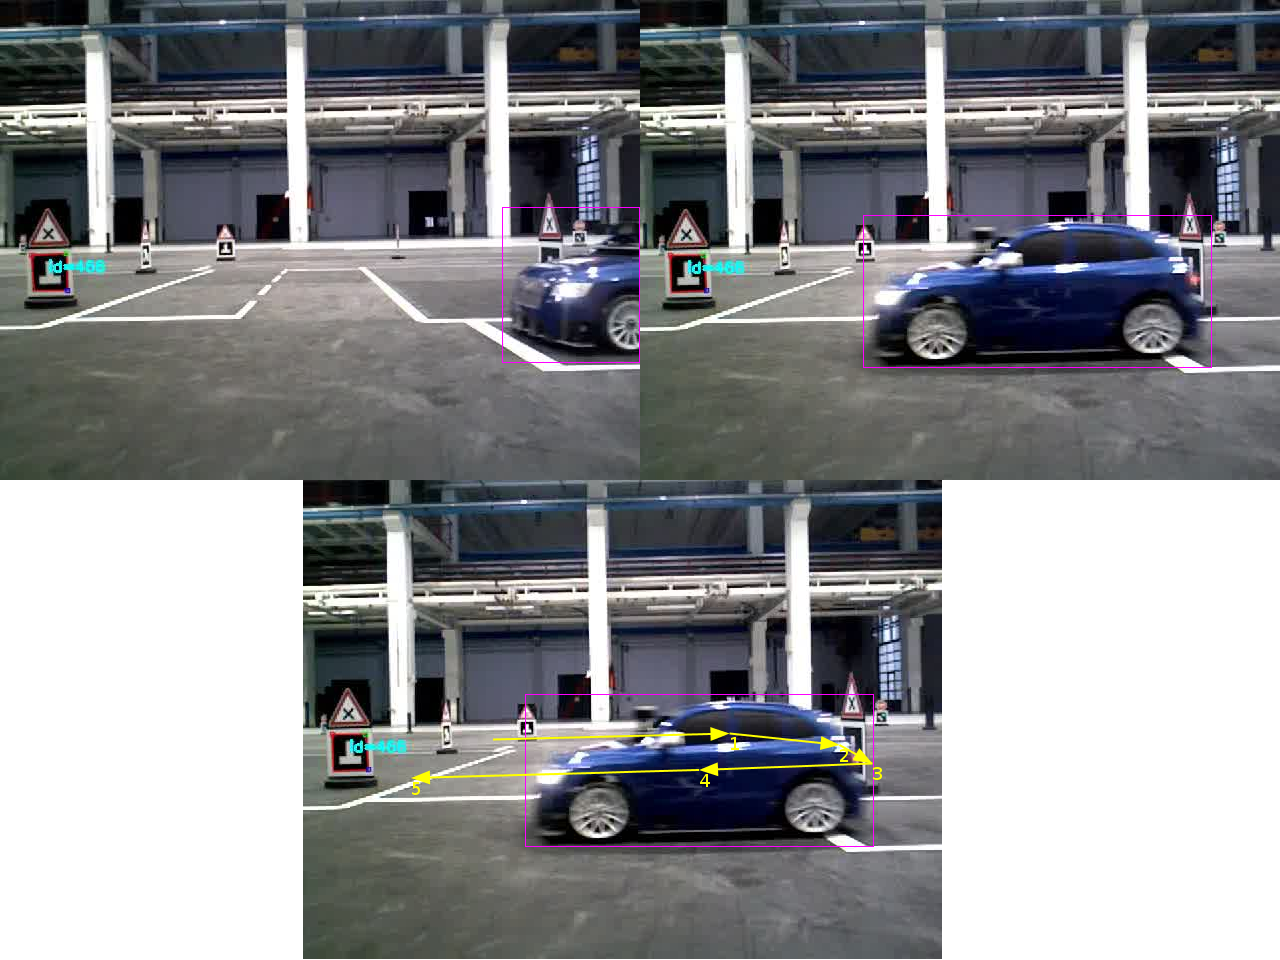
\includegraphics[scale=0.2]{./Abbildungen/08.png}
	\label{img:bsp4}
	\end{figure}

\end{frame}

\section{Verworfene Idee}
\begin{frame}{\secname}

\begin{itemize}
	\item Lucas-Kanade
	\begin{itemize}
	\item kleine Bewegungen nötig
	\item verfolgt Einzelpunkte
	\item gute/prägnante Features nötig
	\item nicht geeignet für dichten Fluss
	\end{itemize}
\end{itemize}

\end{frame}

\section{Umsetzung}
\begin{frame}{\secname}
	
	\begin{itemize}
	
		\item mittels OpenCV
		\begin{itemize}
			\item JavaCV - Javabindings für OpenCV
			\item eigene Methoden für ImageJ-OpenCV-Interoperabilität
		\end{itemize}
		\item implementiert verschiedene Optische-Fluss-Algorithmen
		%\begin{itemize}
			\\ SparseToDense, Farnebäck, DeepFlow, DIS\footnote{Dense Inverse Search}, DualTVL1
		\item Eingabe: zwei Bilder
		\item Ausgabe: 2D-2D-Vektorfeld
		%\end{itemize}
		
	\end{itemize}		
	
\end{frame}

\section{Fluss-Visualisierung}
\begin{frame}{\secname}

	\begin{itemize}
		\item Vektoren bekommen Farbwert zugewiesen
		\item Wahl der Farbe über Farbrad
	\end{itemize}

		
	\begin{figure}[h]
	%\hskip-1.0cm
	\centering
	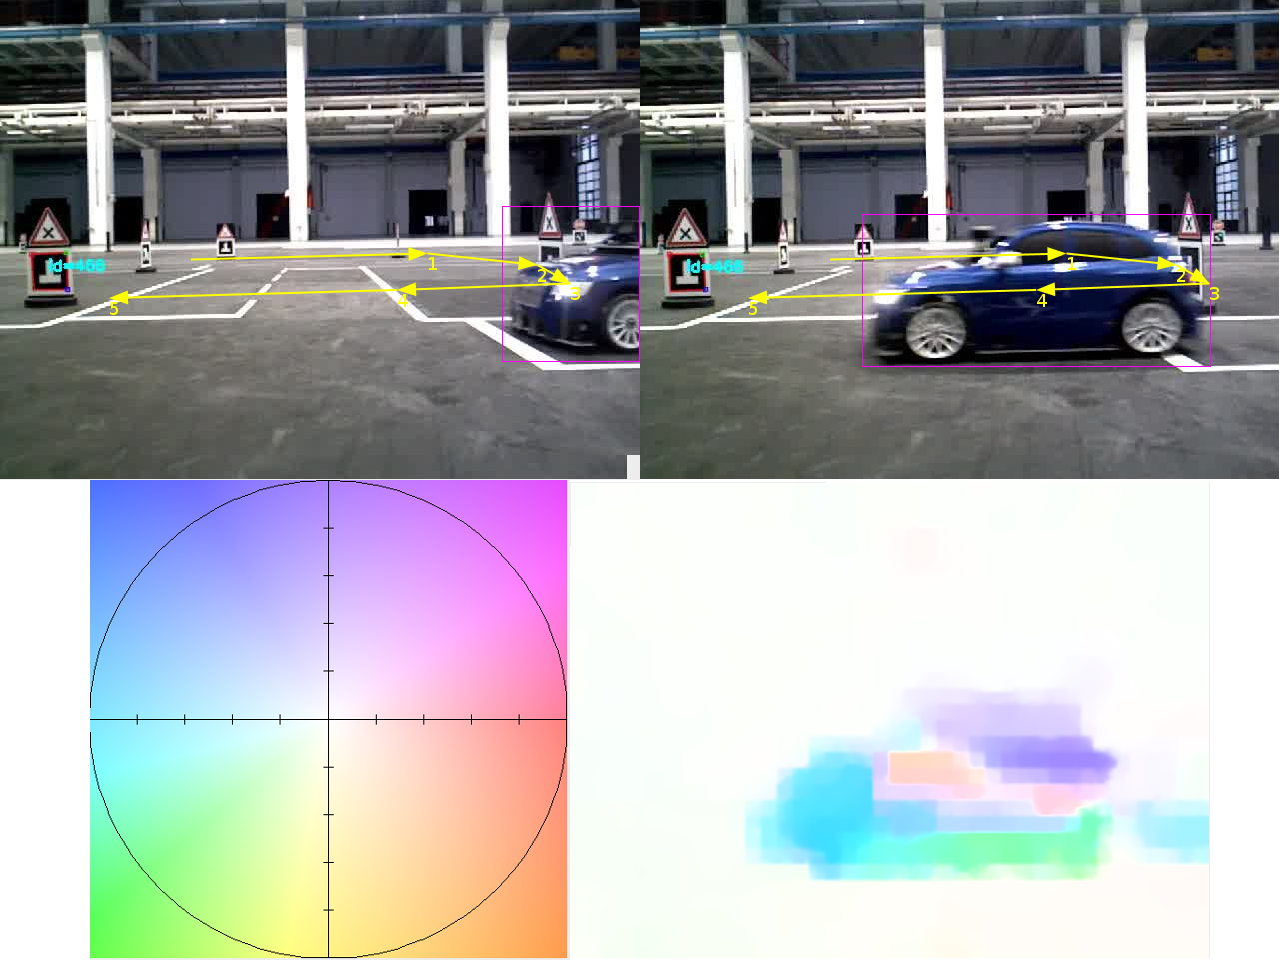
\includegraphics[scale=0.2]{./Abbildungen/7.png}
	\label{img:bsp4}
	\end{figure}

\end{frame}

\section{Aufruf über Kommandozeile}
\begin{frame}{\secname}

\code{ImageJ -macro /flowig/macro/runplug.ijm Flowig\#parameter=<wert>,\dots}

\begin{itemize}
\item \code{path} Pfad zur Bildfolge
\item \code{flow} Algorithmus zur Flussberechnung
  \item \code{showx} und \code{showy} Visualisierung x bzw. y Komponenten

\item\code{boundscolor}: Farbe der Bounding-Boxen

\item\code{maxmotion}: Maximalwert der Farbintensitätsskalierung

\item\code{scalesize}: Anzahl Skalierungen

\item\code{scalecolor}: Sättigungsmultiplikator
\end{itemize}

\end{frame}

\section{Ausblick}
\begin{frame}{\secname}
\begin{itemize}
	\item Entfernen der Ego-Bewegung
	\item Clustern anhand ähnlicher Bewegungsvektoren
	\item um Objekte ohne Bounding-Boxen zu finden
\end{itemize}
\end{frame}

%\section{Zusammenfassung}
%\label{sec_zsf}

%\begin{frame}{\secname}
%Ergebnisse kurz, Ausblick, weitere Themen ausführlicher
%\end{frame}

%\appendix

%\begin{frame}[allowframebreaks]{Quellen}

%  \bibliography{demo}
%  \bibliographystyle{abbrv}

%\end{frame}

\end{document}
